\documentclass[]{article}
\usepackage{lmodern}
\usepackage{amssymb,amsmath}
\usepackage{ifxetex,ifluatex}
\usepackage{fixltx2e} % provides \textsubscript
\ifnum 0\ifxetex 1\fi\ifluatex 1\fi=0 % if pdftex
  \usepackage[T1]{fontenc}
  \usepackage[utf8]{inputenc}
\else % if luatex or xelatex
  \ifxetex
    \usepackage{mathspec}
  \else
    \usepackage{fontspec}
  \fi
  \defaultfontfeatures{Ligatures=TeX,Scale=MatchLowercase}
\fi
% use upquote if available, for straight quotes in verbatim environments
\IfFileExists{upquote.sty}{\usepackage{upquote}}{}
% use microtype if available
\IfFileExists{microtype.sty}{%
\usepackage{microtype}
\UseMicrotypeSet[protrusion]{basicmath} % disable protrusion for tt fonts
}{}
\usepackage[margin=2.54cm]{geometry}
\usepackage{hyperref}
\hypersetup{unicode=true,
            pdftitle={10: Data Visualization},
            pdfauthor={Environmental Data Analytics \textbar{} Kateri Salk},
            pdfborder={0 0 0},
            breaklinks=true}
\urlstyle{same}  % don't use monospace font for urls
\usepackage{color}
\usepackage{fancyvrb}
\newcommand{\VerbBar}{|}
\newcommand{\VERB}{\Verb[commandchars=\\\{\}]}
\DefineVerbatimEnvironment{Highlighting}{Verbatim}{commandchars=\\\{\}}
% Add ',fontsize=\small' for more characters per line
\usepackage{framed}
\definecolor{shadecolor}{RGB}{248,248,248}
\newenvironment{Shaded}{\begin{snugshade}}{\end{snugshade}}
\newcommand{\KeywordTok}[1]{\textcolor[rgb]{0.13,0.29,0.53}{\textbf{#1}}}
\newcommand{\DataTypeTok}[1]{\textcolor[rgb]{0.13,0.29,0.53}{#1}}
\newcommand{\DecValTok}[1]{\textcolor[rgb]{0.00,0.00,0.81}{#1}}
\newcommand{\BaseNTok}[1]{\textcolor[rgb]{0.00,0.00,0.81}{#1}}
\newcommand{\FloatTok}[1]{\textcolor[rgb]{0.00,0.00,0.81}{#1}}
\newcommand{\ConstantTok}[1]{\textcolor[rgb]{0.00,0.00,0.00}{#1}}
\newcommand{\CharTok}[1]{\textcolor[rgb]{0.31,0.60,0.02}{#1}}
\newcommand{\SpecialCharTok}[1]{\textcolor[rgb]{0.00,0.00,0.00}{#1}}
\newcommand{\StringTok}[1]{\textcolor[rgb]{0.31,0.60,0.02}{#1}}
\newcommand{\VerbatimStringTok}[1]{\textcolor[rgb]{0.31,0.60,0.02}{#1}}
\newcommand{\SpecialStringTok}[1]{\textcolor[rgb]{0.31,0.60,0.02}{#1}}
\newcommand{\ImportTok}[1]{#1}
\newcommand{\CommentTok}[1]{\textcolor[rgb]{0.56,0.35,0.01}{\textit{#1}}}
\newcommand{\DocumentationTok}[1]{\textcolor[rgb]{0.56,0.35,0.01}{\textbf{\textit{#1}}}}
\newcommand{\AnnotationTok}[1]{\textcolor[rgb]{0.56,0.35,0.01}{\textbf{\textit{#1}}}}
\newcommand{\CommentVarTok}[1]{\textcolor[rgb]{0.56,0.35,0.01}{\textbf{\textit{#1}}}}
\newcommand{\OtherTok}[1]{\textcolor[rgb]{0.56,0.35,0.01}{#1}}
\newcommand{\FunctionTok}[1]{\textcolor[rgb]{0.00,0.00,0.00}{#1}}
\newcommand{\VariableTok}[1]{\textcolor[rgb]{0.00,0.00,0.00}{#1}}
\newcommand{\ControlFlowTok}[1]{\textcolor[rgb]{0.13,0.29,0.53}{\textbf{#1}}}
\newcommand{\OperatorTok}[1]{\textcolor[rgb]{0.81,0.36,0.00}{\textbf{#1}}}
\newcommand{\BuiltInTok}[1]{#1}
\newcommand{\ExtensionTok}[1]{#1}
\newcommand{\PreprocessorTok}[1]{\textcolor[rgb]{0.56,0.35,0.01}{\textit{#1}}}
\newcommand{\AttributeTok}[1]{\textcolor[rgb]{0.77,0.63,0.00}{#1}}
\newcommand{\RegionMarkerTok}[1]{#1}
\newcommand{\InformationTok}[1]{\textcolor[rgb]{0.56,0.35,0.01}{\textbf{\textit{#1}}}}
\newcommand{\WarningTok}[1]{\textcolor[rgb]{0.56,0.35,0.01}{\textbf{\textit{#1}}}}
\newcommand{\AlertTok}[1]{\textcolor[rgb]{0.94,0.16,0.16}{#1}}
\newcommand{\ErrorTok}[1]{\textcolor[rgb]{0.64,0.00,0.00}{\textbf{#1}}}
\newcommand{\NormalTok}[1]{#1}
\usepackage{graphicx,grffile}
\makeatletter
\def\maxwidth{\ifdim\Gin@nat@width>\linewidth\linewidth\else\Gin@nat@width\fi}
\def\maxheight{\ifdim\Gin@nat@height>\textheight\textheight\else\Gin@nat@height\fi}
\makeatother
% Scale images if necessary, so that they will not overflow the page
% margins by default, and it is still possible to overwrite the defaults
% using explicit options in \includegraphics[width, height, ...]{}
\setkeys{Gin}{width=\maxwidth,height=\maxheight,keepaspectratio}
\IfFileExists{parskip.sty}{%
\usepackage{parskip}
}{% else
\setlength{\parindent}{0pt}
\setlength{\parskip}{6pt plus 2pt minus 1pt}
}
\setlength{\emergencystretch}{3em}  % prevent overfull lines
\providecommand{\tightlist}{%
  \setlength{\itemsep}{0pt}\setlength{\parskip}{0pt}}
\setcounter{secnumdepth}{0}
% Redefines (sub)paragraphs to behave more like sections
\ifx\paragraph\undefined\else
\let\oldparagraph\paragraph
\renewcommand{\paragraph}[1]{\oldparagraph{#1}\mbox{}}
\fi
\ifx\subparagraph\undefined\else
\let\oldsubparagraph\subparagraph
\renewcommand{\subparagraph}[1]{\oldsubparagraph{#1}\mbox{}}
\fi

%%% Use protect on footnotes to avoid problems with footnotes in titles
\let\rmarkdownfootnote\footnote%
\def\footnote{\protect\rmarkdownfootnote}

%%% Change title format to be more compact
\usepackage{titling}

% Create subtitle command for use in maketitle
\newcommand{\subtitle}[1]{
  \posttitle{
    \begin{center}\large#1\end{center}
    }
}

\setlength{\droptitle}{-2em}

  \title{10: Data Visualization}
    \pretitle{\vspace{\droptitle}\centering\huge}
  \posttitle{\par}
    \author{Environmental Data Analytics \textbar{} Kateri Salk}
    \preauthor{\centering\large\emph}
  \postauthor{\par}
      \predate{\centering\large\emph}
  \postdate{\par}
    \date{Spring 2019}


\begin{document}
\maketitle

\subsection{LESSON OBJECTIVES}\label{lesson-objectives}

\begin{enumerate}
\def\labelenumi{\arabic{enumi}.}
\tightlist
\item
  Perform advanced edits on ggplot objects to follow best practices for
  data visualization
\end{enumerate}

\subsection{SET UP YOUR DATA ANALYSIS
SESSION}\label{set-up-your-data-analysis-session}

\begin{Shaded}
\begin{Highlighting}[]
\KeywordTok{getwd}\NormalTok{()}
\end{Highlighting}
\end{Shaded}

\begin{verbatim}
## [1] "C:/Users/Felipe/OneDrive - Duke University/1. DUKE/1. Ramos 2 Semestre/EOS-872 Env. Data Analytics/Environmental_Data_Analytics"
\end{verbatim}

\begin{Shaded}
\begin{Highlighting}[]
\KeywordTok{library}\NormalTok{(tidyverse)}

\NormalTok{PeterPaul.chem.nutrients <-}\StringTok{ }\KeywordTok{read.csv}\NormalTok{(}\StringTok{"./Data/Processed/NTL-LTER_Lake_Chemistry_Nutrients_PeterPaul_Processed.csv"}\NormalTok{)}
\NormalTok{PeterPaul.nutrients.gathered <-}\StringTok{ }\KeywordTok{read.csv}\NormalTok{(}\StringTok{"./Data/Processed/NTL-LTER_Lake_Nutrients_PeterPaulGathered_Processed.csv"}\NormalTok{)}
\NormalTok{EPAair <-}\StringTok{ }\KeywordTok{read.csv}\NormalTok{(}\StringTok{"./Data/Processed/EPAair_O3PM25_3sites1718_processed.csv"}\NormalTok{)}

\NormalTok{EPAair}\OperatorTok{$}\NormalTok{Date <-}\StringTok{ }\KeywordTok{as.Date}\NormalTok{(EPAair}\OperatorTok{$}\NormalTok{Date, }\DataTypeTok{format =} \StringTok{"%Y-%m-%d"}\NormalTok{)}
\NormalTok{PeterPaul.chem.nutrients}\OperatorTok{$}\NormalTok{sampledate <-}\StringTok{ }\KeywordTok{as.Date}\NormalTok{(PeterPaul.chem.nutrients}\OperatorTok{$}\NormalTok{sampledate, }\DataTypeTok{format =} \StringTok{"%Y-%m-%d"}\NormalTok{)}
\end{Highlighting}
\end{Shaded}

\subsubsection{Themes}\label{themes}

Often, we will want to change multiple visual aspects of a plot. Ggplot
comes with pre-built themes that will adjust components of plots if you
call that theme.

\begin{Shaded}
\begin{Highlighting}[]
\NormalTok{O3plot <-}\StringTok{ }\KeywordTok{ggplot}\NormalTok{(EPAair) }\OperatorTok{+}
\StringTok{  }\KeywordTok{geom_point}\NormalTok{(}\KeywordTok{aes}\NormalTok{(}\DataTypeTok{x =}\NormalTok{ Date, }\DataTypeTok{y =}\NormalTok{ Ozone)) }
\KeywordTok{print}\NormalTok{(O3plot)}
\end{Highlighting}
\end{Shaded}

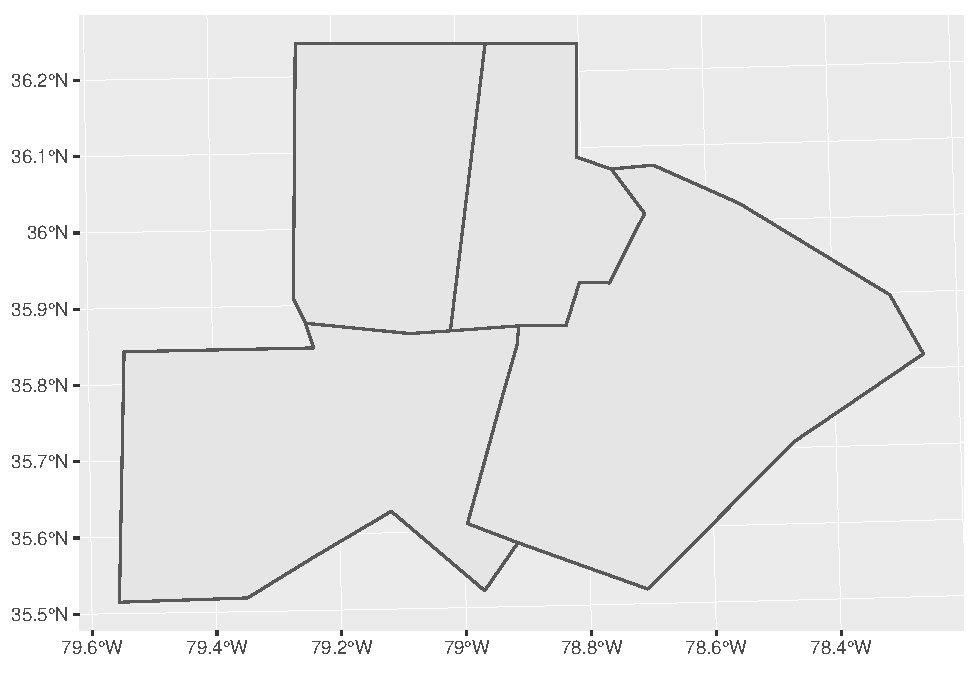
\includegraphics{10_DataVisualization_files/figure-latex/unnamed-chunk-2-1.pdf}

\begin{Shaded}
\begin{Highlighting}[]
\NormalTok{O3plot1 <-}\StringTok{ }\KeywordTok{ggplot}\NormalTok{(EPAair) }\OperatorTok{+}
\StringTok{  }\KeywordTok{geom_point}\NormalTok{(}\KeywordTok{aes}\NormalTok{(}\DataTypeTok{x =}\NormalTok{ Date, }\DataTypeTok{y =}\NormalTok{ Ozone)) }\OperatorTok{+}
\StringTok{  }\KeywordTok{theme_gray}\NormalTok{() }\CommentTok{#default}
\KeywordTok{print}\NormalTok{(O3plot1)}
\end{Highlighting}
\end{Shaded}

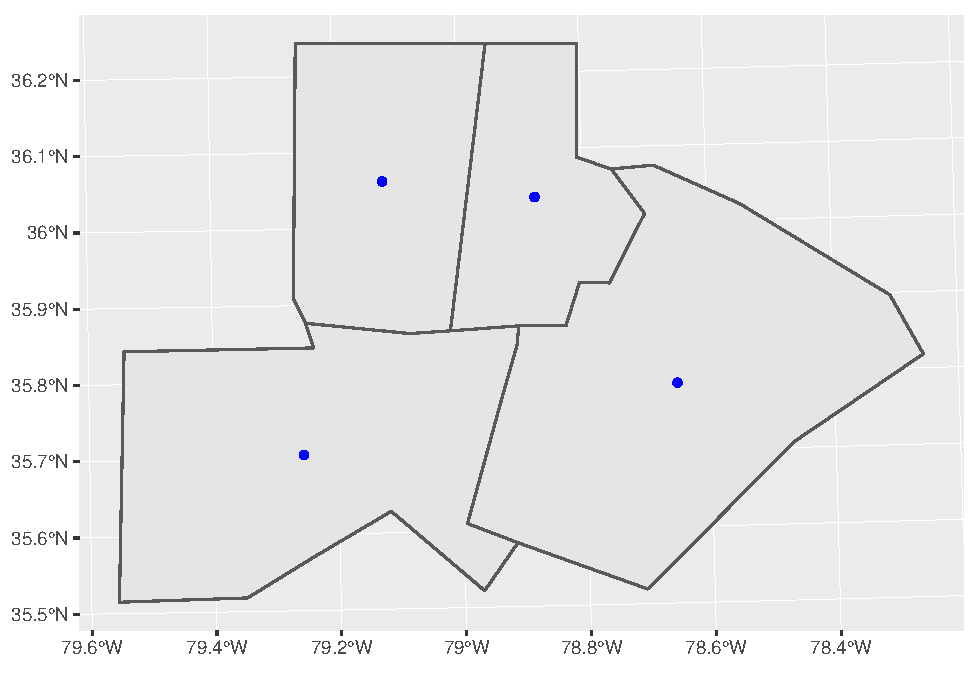
\includegraphics{10_DataVisualization_files/figure-latex/unnamed-chunk-2-2.pdf}

\begin{Shaded}
\begin{Highlighting}[]
\NormalTok{O3plot2 <-}\StringTok{ }\KeywordTok{ggplot}\NormalTok{(EPAair) }\OperatorTok{+}
\StringTok{  }\KeywordTok{geom_point}\NormalTok{(}\KeywordTok{aes}\NormalTok{(}\DataTypeTok{x =}\NormalTok{ Date, }\DataTypeTok{y =}\NormalTok{ Ozone)) }\OperatorTok{+}
\StringTok{  }\KeywordTok{theme_bw}\NormalTok{()}
\KeywordTok{print}\NormalTok{(O3plot2)}
\end{Highlighting}
\end{Shaded}

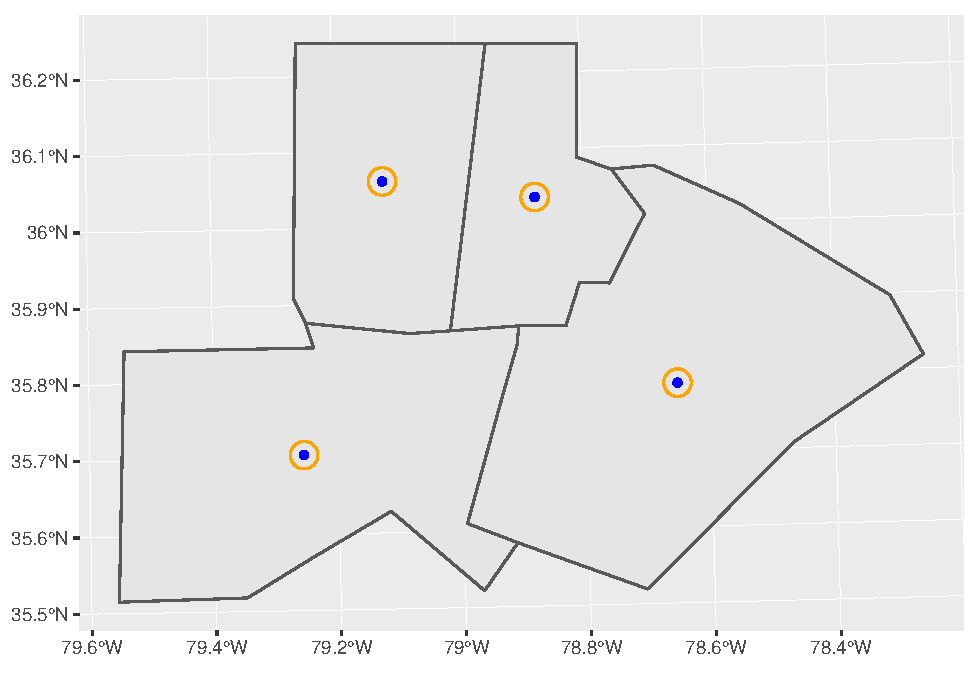
\includegraphics{10_DataVisualization_files/figure-latex/unnamed-chunk-2-3.pdf}

\begin{Shaded}
\begin{Highlighting}[]
\NormalTok{O3plot3 <-}\StringTok{ }\KeywordTok{ggplot}\NormalTok{(EPAair) }\OperatorTok{+}
\StringTok{  }\KeywordTok{geom_point}\NormalTok{(}\KeywordTok{aes}\NormalTok{(}\DataTypeTok{x =}\NormalTok{ Date, }\DataTypeTok{y =}\NormalTok{ Ozone)) }\OperatorTok{+}
\StringTok{  }\KeywordTok{theme_light}\NormalTok{()}
\KeywordTok{print}\NormalTok{(O3plot3)}
\end{Highlighting}
\end{Shaded}

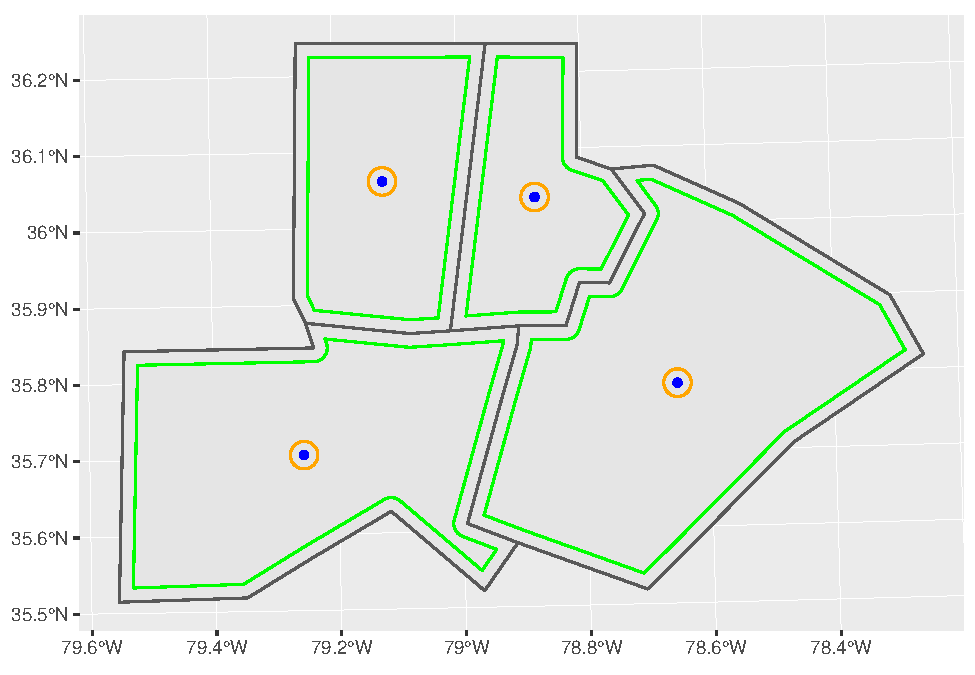
\includegraphics{10_DataVisualization_files/figure-latex/unnamed-chunk-2-4.pdf}

\begin{Shaded}
\begin{Highlighting}[]
\NormalTok{O3plot4 <-}\StringTok{ }\KeywordTok{ggplot}\NormalTok{(EPAair) }\OperatorTok{+}
\StringTok{  }\KeywordTok{geom_point}\NormalTok{(}\KeywordTok{aes}\NormalTok{(}\DataTypeTok{x =}\NormalTok{ Date, }\DataTypeTok{y =}\NormalTok{ Ozone)) }\OperatorTok{+}
\StringTok{  }\KeywordTok{theme_classic}\NormalTok{() }\CommentTok{#Kateri like this one (no grid)}
\KeywordTok{print}\NormalTok{(O3plot4)}
\end{Highlighting}
\end{Shaded}

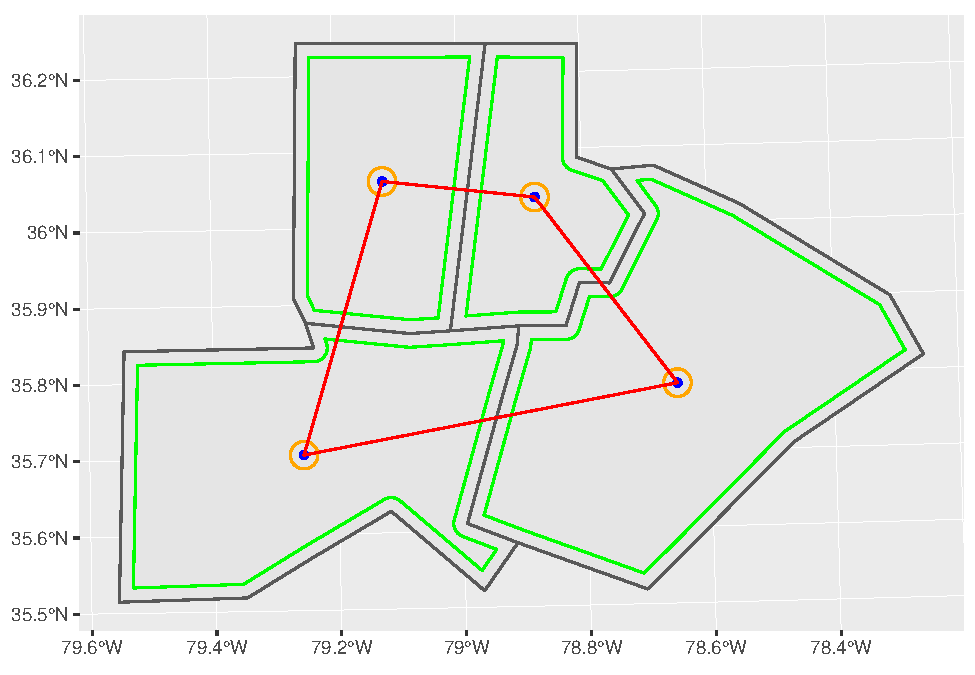
\includegraphics{10_DataVisualization_files/figure-latex/unnamed-chunk-2-5.pdf}

Notice that some aspects of your graph have not been adjusted,
including:

\begin{itemize}
\tightlist
\item
  text size
\item
  axis label colors
\item
  legend position and justification
\end{itemize}

If you would like to set a common theme across all plots in your
analysis session, you may define a theme and call up that theme for each
graph. This eliminates the need to add multiple lines of code in each
plot.

\begin{Shaded}
\begin{Highlighting}[]
\NormalTok{mytheme <-}\StringTok{ }\KeywordTok{theme_classic}\NormalTok{(}\DataTypeTok{base_size =} \DecValTok{14}\NormalTok{) }\OperatorTok{+}\StringTok{ }\CommentTok{#you can put any name}
\StringTok{  }\KeywordTok{theme}\NormalTok{(}\DataTypeTok{axis.text =} \KeywordTok{element_text}\NormalTok{(}\DataTypeTok{color =} \StringTok{"black"}\NormalTok{), }
        \DataTypeTok{legend.position =} \StringTok{"top"}\NormalTok{) }

\CommentTok{# options: call the theme in each plot or set the theme at the start. }

\NormalTok{O3plot5 <-}\StringTok{ }\KeywordTok{ggplot}\NormalTok{(EPAair) }\OperatorTok{+}
\StringTok{  }\KeywordTok{geom_point}\NormalTok{(}\KeywordTok{aes}\NormalTok{(}\DataTypeTok{x =}\NormalTok{ Date, }\DataTypeTok{y =}\NormalTok{ Ozone)) }\OperatorTok{+}
\StringTok{  }\NormalTok{mytheme }\CommentTok{#one way of doing it}
\KeywordTok{print}\NormalTok{(O3plot5)  }
\end{Highlighting}
\end{Shaded}

\includegraphics{10_DataVisualization_files/figure-latex/unnamed-chunk-3-1.pdf}

\begin{Shaded}
\begin{Highlighting}[]
\KeywordTok{theme_set}\NormalTok{(mytheme) }\CommentTok{#this is other way of doing it. Better for several plots.}

\NormalTok{O3plot6 <-}\StringTok{ }\KeywordTok{ggplot}\NormalTok{(EPAair) }\OperatorTok{+}
\StringTok{  }\KeywordTok{geom_point}\NormalTok{(}\KeywordTok{aes}\NormalTok{(}\DataTypeTok{x =}\NormalTok{ Date, }\DataTypeTok{y =}\NormalTok{ Ozone))}
\KeywordTok{print}\NormalTok{(O3plot6)  }
\end{Highlighting}
\end{Shaded}

\includegraphics{10_DataVisualization_files/figure-latex/unnamed-chunk-3-2.pdf}

\subsubsection{Adjusting multiple components of your
plots}\label{adjusting-multiple-components-of-your-plots}

While the theme allows us to set multiple aspects of plots, ggplot
allows us to adjust other parts of plots outside of the theme.

\begin{Shaded}
\begin{Highlighting}[]
\NormalTok{O3plot7 <-}\StringTok{ }\KeywordTok{ggplot}\NormalTok{(EPAair, }\KeywordTok{aes}\NormalTok{(}\DataTypeTok{x =}\NormalTok{ Date, }\DataTypeTok{y =}\NormalTok{ Ozone)) }\OperatorTok{+}
\StringTok{  }\KeywordTok{geom_rect}\NormalTok{(}\DataTypeTok{xmin =} \KeywordTok{as.Date}\NormalTok{(}\StringTok{"2016-01-01"}\NormalTok{), }\DataTypeTok{xmax =} \KeywordTok{as.Date}\NormalTok{(}\StringTok{"2020-01-01"}\NormalTok{),  }\CommentTok{#ojo as.date}
            \DataTypeTok{ymin =} \DecValTok{0}\NormalTok{, }\DataTypeTok{ymax =} \DecValTok{50}\NormalTok{, }\DataTypeTok{fill =} \StringTok{"green"}\NormalTok{) }\OperatorTok{+}
\StringTok{  }\KeywordTok{geom_rect}\NormalTok{(}\DataTypeTok{xmin =} \KeywordTok{as.Date}\NormalTok{(}\StringTok{"2016-01-01"}\NormalTok{), }\DataTypeTok{xmax =} \KeywordTok{as.Date}\NormalTok{(}\StringTok{"2020-01-01"}\NormalTok{), }
            \DataTypeTok{ymin =} \DecValTok{50}\NormalTok{, }\DataTypeTok{ymax =} \DecValTok{100}\NormalTok{, }\DataTypeTok{fill =} \StringTok{"yellow"}\NormalTok{) }\OperatorTok{+}
\StringTok{  }\KeywordTok{geom_point}\NormalTok{() }\OperatorTok{+}\StringTok{ }\CommentTok{#first geom_rect than points}
\StringTok{  }\KeywordTok{geom_text}\NormalTok{(}\DataTypeTok{x =} \KeywordTok{as.Date}\NormalTok{(}\StringTok{"2019-01-01"}\NormalTok{), }\DataTypeTok{y =} \DecValTok{45}\NormalTok{, }\DataTypeTok{label =} \StringTok{"good"}\NormalTok{, }\DataTypeTok{hjust =} \DecValTok{1}\NormalTok{, }\DataTypeTok{fontface =} \StringTok{"bold"}\NormalTok{) }\OperatorTok{+}
\StringTok{  }\KeywordTok{geom_text}\NormalTok{(}\DataTypeTok{x =} \KeywordTok{as.Date}\NormalTok{(}\StringTok{"2019-01-01"}\NormalTok{), }\DataTypeTok{y =} \DecValTok{95}\NormalTok{, }\DataTypeTok{label =} \StringTok{"moderate"}\NormalTok{, }\DataTypeTok{hjust =} \DecValTok{1}\NormalTok{, }\DataTypeTok{fontface =} \StringTok{"bold"}\NormalTok{) }\OperatorTok{+}
\StringTok{  }\KeywordTok{scale_x_date}\NormalTok{(}\DataTypeTok{limits =} \KeywordTok{as.Date}\NormalTok{(}\KeywordTok{c}\NormalTok{(}\StringTok{"2017-01-01"}\NormalTok{, }\StringTok{"2018-12-31"}\NormalTok{)), }
    \DataTypeTok{date_breaks =} \StringTok{"2 months"}\NormalTok{, }\DataTypeTok{date_labels =} \StringTok{"%b %y"}\NormalTok{) }\OperatorTok{+}
\StringTok{  }\KeywordTok{ylab}\NormalTok{(}\KeywordTok{expression}\NormalTok{(}\StringTok{"O"}\NormalTok{[}\DecValTok{3}\NormalTok{]}\OperatorTok{*}\StringTok{ " AQI Value"}\NormalTok{)) }\OperatorTok{+}
\StringTok{  }\KeywordTok{theme}\NormalTok{(}\DataTypeTok{axis.text.x =} \KeywordTok{element_text}\NormalTok{(}\DataTypeTok{angle =} \DecValTok{45}\NormalTok{,  }\DataTypeTok{hjust =} \DecValTok{1}\NormalTok{)) }\CommentTok{#this theme only changes the things you specify}
\KeywordTok{print}\NormalTok{(O3plot7)  }
\end{Highlighting}
\end{Shaded}

\includegraphics{10_DataVisualization_files/figure-latex/unnamed-chunk-4-1.pdf}

\subsubsection{Color palettes}\label{color-palettes}

There are several color palettes that are designed to be more effective
than palettes in base R. These include Viridis
(\url{https://cran.r-project.org/web/packages/viridis/vignettes/intro-to-viridis.html})
and Color Brewer (\url{http://colorbrewer2.org/}). A few rules for
choosing colors:

\begin{itemize}
\tightlist
\item
  Consider if your plot needs to be viewed in black and white. If so,
  choose a sequential palette with varying color intensity.
\item
  Choose a palette that is color-blind friendly
\item
  Maximize contrast (e.g., no pale colors on a white background)
\item
  Diverging color palettes should be used for diverging values (e.g.,
  warm-to-cool works well for values on a scale encompassing negative
  and positive values)
\end{itemize}

Perception is key! Choose palettes that are visually pleasing and will
communicate what you are hoping your audience to perceive. Hint: base R
palettes are not ideal.

\begin{Shaded}
\begin{Highlighting}[]
\CommentTok{#install.packages("viridis")    #####use always in the beginign}
\CommentTok{#install.packages("RColorBrewer")}
\CommentTok{#install.packages("colormap")}
\KeywordTok{library}\NormalTok{(viridis)}
\end{Highlighting}
\end{Shaded}

\begin{verbatim}
## Loading required package: viridisLite
\end{verbatim}

\begin{Shaded}
\begin{Highlighting}[]
\KeywordTok{library}\NormalTok{(RColorBrewer)}
\KeywordTok{library}\NormalTok{(colormap)}

\NormalTok{scales}\OperatorTok{::}\KeywordTok{show_col}\NormalTok{(}\KeywordTok{colormap}\NormalTok{(}\DataTypeTok{colormap =}\NormalTok{ colormaps}\OperatorTok{$}\NormalTok{viridis, }\DataTypeTok{nshades =} \DecValTok{16}\NormalTok{))}
\end{Highlighting}
\end{Shaded}

\includegraphics{10_DataVisualization_files/figure-latex/unnamed-chunk-5-1.pdf}

\begin{Shaded}
\begin{Highlighting}[]
\NormalTok{scales}\OperatorTok{::}\KeywordTok{show_col}\NormalTok{(}\KeywordTok{colormap}\NormalTok{(}\DataTypeTok{colormap =}\NormalTok{ colormaps}\OperatorTok{$}\NormalTok{inferno, }\DataTypeTok{nshades =} \DecValTok{16}\NormalTok{))}
\end{Highlighting}
\end{Shaded}

\includegraphics{10_DataVisualization_files/figure-latex/unnamed-chunk-5-2.pdf}

\begin{Shaded}
\begin{Highlighting}[]
\NormalTok{scales}\OperatorTok{::}\KeywordTok{show_col}\NormalTok{(}\KeywordTok{colormap}\NormalTok{(}\DataTypeTok{colormap =}\NormalTok{ colormaps}\OperatorTok{$}\NormalTok{magma, }\DataTypeTok{nshades =} \DecValTok{16}\NormalTok{))}
\end{Highlighting}
\end{Shaded}

\includegraphics{10_DataVisualization_files/figure-latex/unnamed-chunk-5-3.pdf}

\begin{Shaded}
\begin{Highlighting}[]
\KeywordTok{display.brewer.all}\NormalTok{(}\DataTypeTok{n =} \DecValTok{9}\NormalTok{) }\CommentTok{# from the website you cna use. color blind!!!!}
\end{Highlighting}
\end{Shaded}

\includegraphics{10_DataVisualization_files/figure-latex/unnamed-chunk-5-4.pdf}

\begin{Shaded}
\begin{Highlighting}[]
\NormalTok{NvsP <-}
\StringTok{  }\KeywordTok{ggplot}\NormalTok{(PeterPaul.chem.nutrients, }\KeywordTok{aes}\NormalTok{(}\DataTypeTok{x =}\NormalTok{ tp_ug, }\DataTypeTok{y =}\NormalTok{ tn_ug, }\DataTypeTok{color =}\NormalTok{ depth, }\DataTypeTok{shape =}\NormalTok{ lakename)) }\OperatorTok{+}
\StringTok{  }\KeywordTok{geom_point}\NormalTok{() }
\KeywordTok{print}\NormalTok{(NvsP)}
\end{Highlighting}
\end{Shaded}

\includegraphics{10_DataVisualization_files/figure-latex/unnamed-chunk-5-5.pdf}

\begin{Shaded}
\begin{Highlighting}[]
\CommentTok{# let's first make the plot look better.}
\CommentTok{# change your axis labels to reflect TN and TP in micrograms per liter.}
\CommentTok{# change your legend labels}
\NormalTok{NvsP2 <-}
\StringTok{  }\KeywordTok{ggplot}\NormalTok{(PeterPaul.chem.nutrients, }\KeywordTok{aes}\NormalTok{(}\DataTypeTok{x =}\NormalTok{ tp_ug, }\DataTypeTok{y =}\NormalTok{ tn_ug, }\DataTypeTok{color =}\NormalTok{ depth, }\DataTypeTok{shape =}\NormalTok{ lakename)) }\OperatorTok{+}
\StringTok{  }\KeywordTok{geom_point}\NormalTok{(}\DataTypeTok{alpha =} \FloatTok{0.8}\NormalTok{, }\DataTypeTok{size =} \DecValTok{3}\NormalTok{) }\OperatorTok{+}
\StringTok{  }\KeywordTok{xlab}\NormalTok{(}\KeywordTok{expression}\NormalTok{(}\StringTok{"Total Phosphorus, (\textbackslash{}U003BCg/lt)"}\NormalTok{)) }\OperatorTok{+}\StringTok{ }\CommentTok{#there are codes for greek leters}
\StringTok{  }\KeywordTok{ylab}\NormalTok{(}\KeywordTok{expression}\NormalTok{(}\StringTok{"Total Nitrogen (\textbackslash{}U003BCg/lt)"}\NormalTok{)) }\OperatorTok{+}
\StringTok{  }\CommentTok{# change your legend labels here}
\StringTok{  }\KeywordTok{scale_shape_manual}\NormalTok{(}\DataTypeTok{values =} \KeywordTok{c}\NormalTok{(}\DecValTok{15}\NormalTok{, }\DecValTok{17}\NormalTok{)) }\OperatorTok{+}
\StringTok{ }\CommentTok{# scale_color_distiller(palette = "Blues", direction = 1) + # use scale_color_brewer for discrete variables}
\StringTok{  }\KeywordTok{scale_color_viridis}\NormalTok{(}\DataTypeTok{option =} \StringTok{"magma"}\NormalTok{, }\DataTypeTok{direction =} \OperatorTok{-}\DecValTok{1}\NormalTok{) }\OperatorTok{+}
\StringTok{  }\KeywordTok{theme}\NormalTok{(}\DataTypeTok{legend.position =} \StringTok{"right"}\NormalTok{, }
        \DataTypeTok{legend.text =} \KeywordTok{element_text}\NormalTok{(}\DataTypeTok{size =} \DecValTok{12}\NormalTok{), }\DataTypeTok{legend.title =} \KeywordTok{element_text}\NormalTok{(}\DataTypeTok{size =} \DecValTok{12}\NormalTok{))}
\KeywordTok{print}\NormalTok{(NvsP2)  }\CommentTok{#change legend titles (we tried to do it)}
\end{Highlighting}
\end{Shaded}

\includegraphics{10_DataVisualization_files/figure-latex/unnamed-chunk-5-6.pdf}

\begin{Shaded}
\begin{Highlighting}[]
\CommentTok{# change your y axis label to list concentration in micrograms per liter}
\CommentTok{# remove your x axis label}
\CommentTok{# change labels for nutrients in the legend}

\NormalTok{Nutrientplot <-}
\StringTok{  }\KeywordTok{ggplot}\NormalTok{(PeterPaul.nutrients.gathered, }\KeywordTok{aes}\NormalTok{(}\DataTypeTok{x =}\NormalTok{ lakename, }\DataTypeTok{y =}\NormalTok{ concentration, }\DataTypeTok{color =}\NormalTok{ nutrient)) }\OperatorTok{+}
\StringTok{  }\KeywordTok{geom_boxplot}\NormalTok{() }\OperatorTok{+}
\CommentTok{# place your additional edits here}
\StringTok{  }\KeywordTok{scale_y_continuous}\NormalTok{(}\DataTypeTok{expand =} \KeywordTok{c}\NormalTok{(}\DecValTok{0}\NormalTok{, }\DecValTok{0}\NormalTok{)) }\OperatorTok{+}
\StringTok{  }\CommentTok{#scale_color_brewer(palette = "YlGnBu") +}
\StringTok{  }\KeywordTok{scale_color_manual}\NormalTok{(}\DataTypeTok{values =} \KeywordTok{c}\NormalTok{(}\StringTok{"#7fcdbb"}\NormalTok{, }\StringTok{"#41b6c4"}\NormalTok{, }\StringTok{"#1d91c0"}\NormalTok{, }\StringTok{"#225ea8"}\NormalTok{, }\StringTok{"#0c2c84"}\NormalTok{)) }\OperatorTok{+}\StringTok{ }\CommentTok{#from the website}
\StringTok{  }\CommentTok{#scale_color_viridis(discrete = TRUE) + #another option. problem with the yellow.}
\StringTok{  }\KeywordTok{theme}\NormalTok{(}\DataTypeTok{legend.position =} \StringTok{"right"}\NormalTok{) }\OperatorTok{+}
\StringTok{  }\KeywordTok{ylab}\NormalTok{(}\KeywordTok{expression}\NormalTok{(}\StringTok{"Concentration (\textbackslash{}U003BCg/lt)"}\NormalTok{)) }\OperatorTok{+}
\StringTok{  }\KeywordTok{xlab}\NormalTok{(}\KeywordTok{expression}\NormalTok{(}\StringTok{""}\NormalTok{))}

\KeywordTok{print}\NormalTok{(Nutrientplot)}
\end{Highlighting}
\end{Shaded}

\includegraphics{10_DataVisualization_files/figure-latex/unnamed-chunk-5-7.pdf}

\subsubsection{Adjusting facets}\label{adjusting-facets}

\begin{Shaded}
\begin{Highlighting}[]
\NormalTok{PMplot.faceted <-}
\StringTok{  }\KeywordTok{ggplot}\NormalTok{(EPAair, }\KeywordTok{aes}\NormalTok{(}\DataTypeTok{x =}\NormalTok{ month, }\DataTypeTok{y =}\NormalTok{ PM2.}\DecValTok{5}\NormalTok{)) }\OperatorTok{+}
\StringTok{  }\KeywordTok{geom_point}\NormalTok{() }\OperatorTok{+}
\StringTok{  }\KeywordTok{facet_grid}\NormalTok{(Site.Name }\OperatorTok{~}\StringTok{ }\NormalTok{year) }\OperatorTok{+}\StringTok{ }
\StringTok{  }\KeywordTok{scale_x_continuous}\NormalTok{(}\DataTypeTok{breaks =} \KeywordTok{c}\NormalTok{(}\DecValTok{1}\OperatorTok{:}\DecValTok{12}\NormalTok{)) }\OperatorTok{+}
\StringTok{  }\KeywordTok{theme}\NormalTok{(}\DataTypeTok{strip.background =} \KeywordTok{element_rect}\NormalTok{(}\DataTypeTok{fill =} \StringTok{"black"}\NormalTok{), }\DataTypeTok{strip.text =} \KeywordTok{element_text}\NormalTok{(}\DataTypeTok{color =} \StringTok{"white"}\NormalTok{)) }\OperatorTok{+}
\StringTok{  }\KeywordTok{ylab}\NormalTok{(}\KeywordTok{expression}\NormalTok{(}\StringTok{"PM 2.5 AQI Value"}\NormalTok{)) }
\KeywordTok{print}\NormalTok{(PMplot.faceted)}
\end{Highlighting}
\end{Shaded}

\begin{verbatim}
## Warning: Removed 52 rows containing missing values (geom_point).
\end{verbatim}

\includegraphics{10_DataVisualization_files/figure-latex/unnamed-chunk-6-1.pdf}

\subsubsection{Multiple plots on a page}\label{multiple-plots-on-a-page}

In situations where facets don't fill our needs to place multiple plots
on a page, we can use the package \texttt{gridExtra} to arrange plots.
The \texttt{grid.arrange} function is extremely flexible in its ability
to arrange plots in specific configurations. A useful guide can be found
here:
\url{https://cran.r-project.org/web/packages/egg/vignettes/Ecosystem.html}.

\begin{Shaded}
\begin{Highlighting}[]
\CommentTok{#install.packages("gridExtra")}
\KeywordTok{library}\NormalTok{(gridExtra)}
\end{Highlighting}
\end{Shaded}

\begin{verbatim}
## 
## Attaching package: 'gridExtra'
\end{verbatim}

\begin{verbatim}
## The following object is masked from 'package:dplyr':
## 
##     combine
\end{verbatim}

\begin{Shaded}
\begin{Highlighting}[]
\KeywordTok{grid.arrange}\NormalTok{(NvsP2, Nutrientplot)}
\end{Highlighting}
\end{Shaded}

\begin{verbatim}
## Warning: Removed 21648 rows containing missing values (geom_point).
\end{verbatim}

\includegraphics{10_DataVisualization_files/figure-latex/unnamed-chunk-7-1.pdf}

\begin{Shaded}
\begin{Highlighting}[]
\KeywordTok{grid.arrange}\NormalTok{(O3plot7, PMplot.faceted)}
\end{Highlighting}
\end{Shaded}

\begin{verbatim}
## Warning: Removed 868 rows containing missing values (geom_point).
\end{verbatim}

\begin{verbatim}
## Warning: Removed 52 rows containing missing values (geom_point).
\end{verbatim}

\includegraphics{10_DataVisualization_files/figure-latex/unnamed-chunk-7-2.pdf}

\subsubsection{Saving plots \#reprodusable
way}\label{saving-plots-reprodusable-way}

The \texttt{ggsave} function allows you to save plots in jpg, png, eps,
pdf, tiff, and other formats. The following information can be supplied:

\begin{itemize}
\tightlist
\item
  filename, with file extension and in quotes (required)
\item
  plot object (required)
\item
  path, with file name
\item
  width, height, units
\item
  resolution (dpi)
\end{itemize}

For example:
\texttt{ggsave("PMplot.jpg",\ PMplot.faceted,\ \ path\ =\ "./Output/PMplot.jpg",\ height\ =\ 4,\ width\ =\ 6,\ units\ =\ "in",\ dpi\ =\ 300)}


\end{document}
